%! Date = 2/22/24

\section{Introduction}\label{sec:introduction}
%Larger Transformer~\cite{NEURIPS2017_3f5ee243} models achieve significantly better performance
%~\cite{DBLP:journals/corr/abs-2005-14165},
%hence the appeal for continuous scale.
%However, this increase in model size demands exorbitant compute resources,
%necessitating a distributed setting as memory requirements exceed the capacity of any
%accelerator~\cite{DBLP:journals/corr/abs-2201-11990}
%This interplay asks:
%\emph{how do we sidestep the high costs of scaling Large Transformer models?}
%Although highly efficient for scaling~\cite{pmlr-v162-rajbhandari22a, Gemini_Team_2024},
%the Mixture-of-Experts (MoE) architecture~\cite{ShazeerMMDLHD17},
%based on ~\emph{conditional computation}~\cite{doi:10.1142/S0218001403002411},
%introduces unsolved algorithmic and systems challenges,
%such as load balancing across experts~\cite{ShazeerMMDLHD17},
%expert capacity restriction leading to token dropping~\cite{DBLP:journals/corr/abs-2101-03961},
%and collective communication overhead~\cite{DBLP:journals/corr/abs-2006-16668}.
\begin{figure}[!h]
    \begin{subfigure}{.5\linewidth}
        \centering
        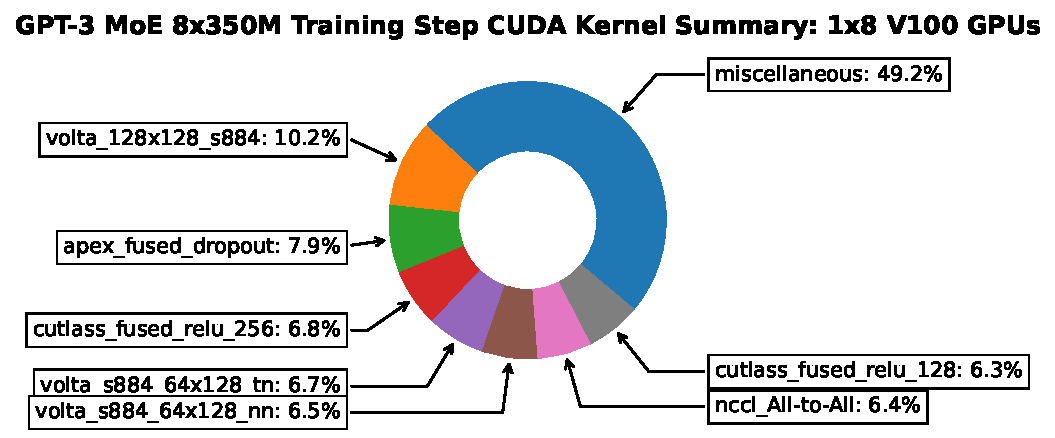
\includegraphics[width=\linewidth]{images/single_trace_1x8_donut}
        \caption{NDv2 Node}
        \label{singlepie}
    \end{subfigure}\hfill % <-- "\hfill"
    \begin{subfigure}{.5\linewidth}
        \centering
        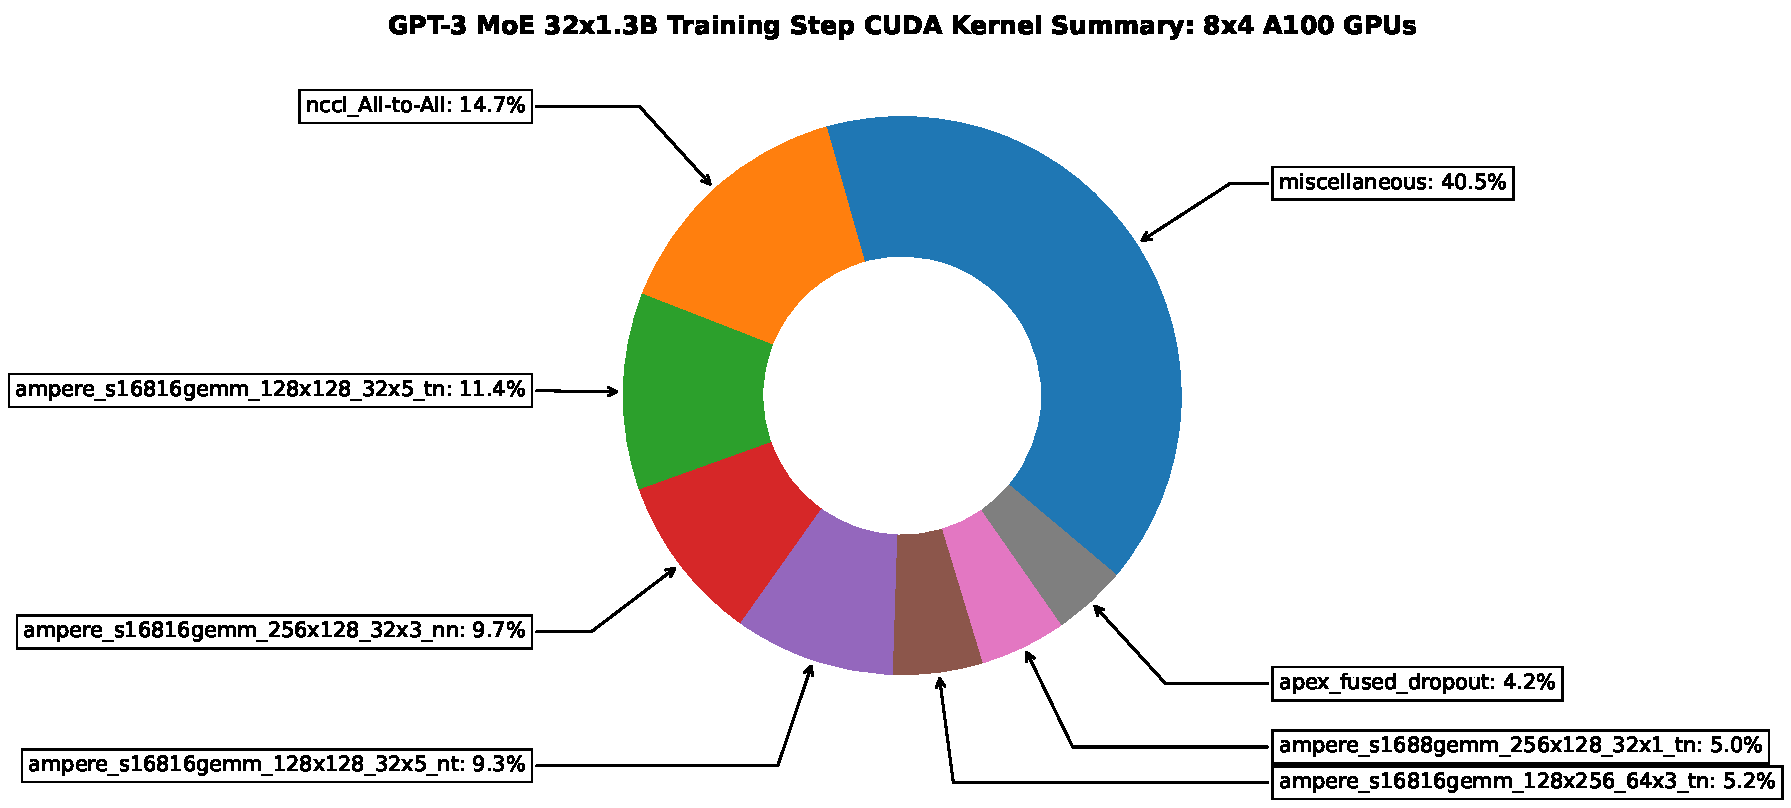
\includegraphics[width=\linewidth]{images/multi_sum_8x4_1.3B_donut}
        \caption{8 Perlmutter GPU Nodes}
        \label{multi_1.3B_pie}
    \end{subfigure}
    \caption{\footnotesize DMoE Training Step CUDA Kernel Distribution.
    Observe in \ref{multi_1.3B_pie} that \emph{All-to-All} is the single most expensive operation.
    Note Perlmutter is a supercomputer. $W$x350M means a 350M model with $W$ experts, where each GPU hosts one expert}
    \label{fig:donut}
\end{figure}

\begin{figure}[!ht]
    \begin{subfigure}{.5\linewidth}
        \centering
        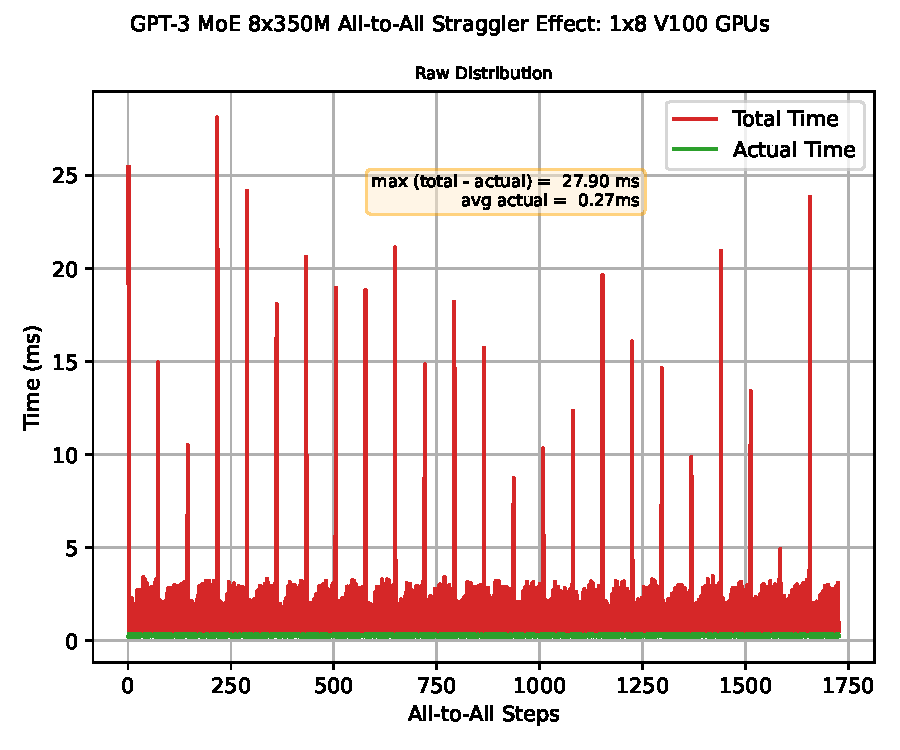
\includegraphics[width=0.6\linewidth, keepaspectratio]{images/GPT-3_MoE_8x350M}
        \caption{NDv2}
        \label{sub:s_350}
    \end{subfigure}\hfill % <-- "\hfill"
    \begin{subfigure}{.5\linewidth}
        \centering
        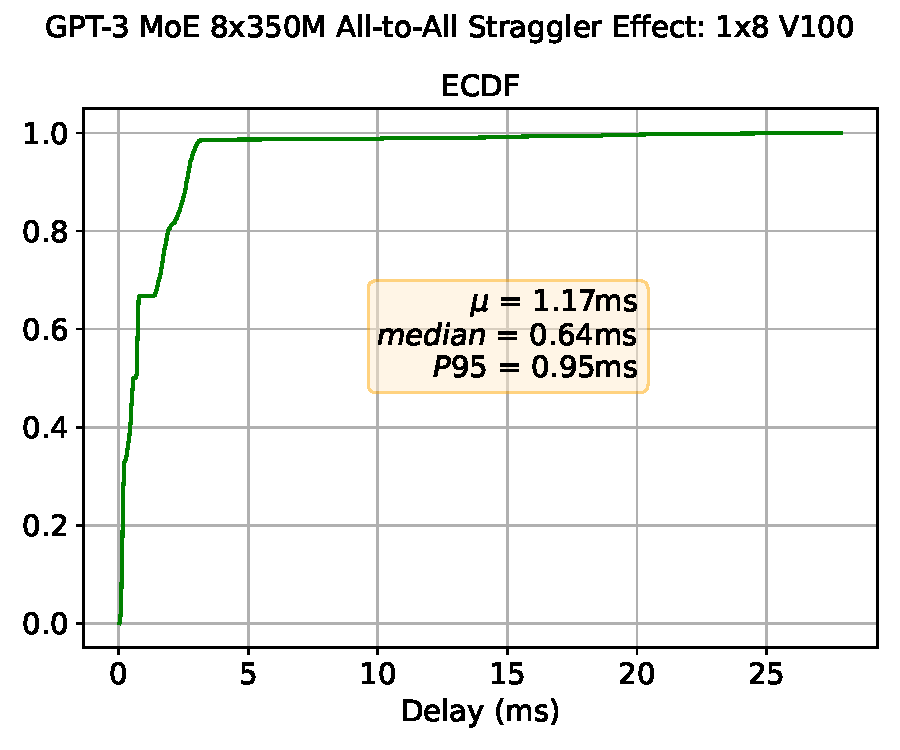
\includegraphics[width=0.6\linewidth, keepaspectratio]{images/GPT-3_MoE_8x350M_ecdf}
        \caption{NDv2 ECDF}
        \label{sub:s_350_ecdf}
    \end{subfigure}
    \smallskip % create some *vertical* separation between the graphs
    \begin{subfigure}{.5\linewidth}
        \centering
        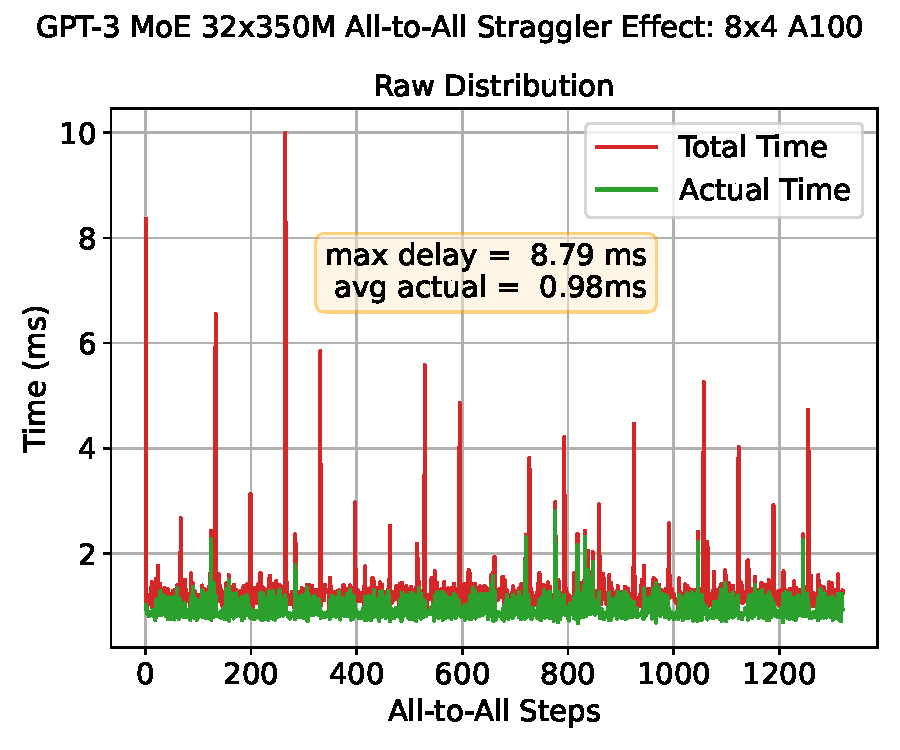
\includegraphics[width=0.6\linewidth, keepaspectratio]{images/GPT-3_MoE_32x350M}
        \caption{8x4 GPUs}
        \label{sub:m_350}
    \end{subfigure}\hfill % <-- "\hfill"
    \begin{subfigure}{.5\linewidth}
        \centering
        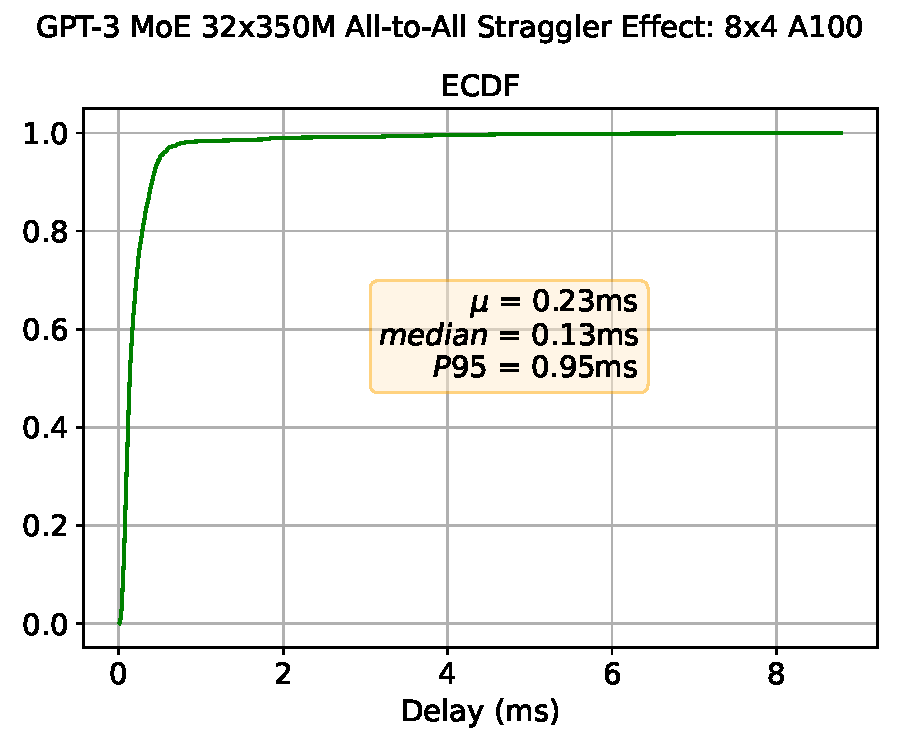
\includegraphics[width=0.6\linewidth, keepaspectratio]{images/GPT-3_MoE_32x350M_ecdf}
        \caption{8x4 GPUs ECDF}
        \label{sub:m_350_ecdf}
    \end{subfigure}
    \caption{\footnotesize Straggler Effect in DMoE Training.
    \textbf{Actual Time} $t_a$ denotes time for the slowest worker to complete the kernel,
        while \textbf{Total Time} $t$ includes the time the fastest worker had to \emph{wait}.
        Note $Delay = t - t_a$ and $\mu$ denotes mean.}
    \label{fig:straggler}
\end{figure}
In this work
~\footnote{\href{https://github.com/osayamenja/DataCruncher}{Notebook} for all plots and traces and
\href{https://github.com/osayamenja/Megatron-DeepSpeed}{Training Code}},
we focus on the overhead of synchronous \emph{All-to-All},
within Distributed MoE~\cite{DBLP:journals/corr/abs-2006-16668}
and make the following contributions.
Firstly, we empirically demonstrate that the synchronous constraint of \verb|All-to-All|
as implemented by NCCL degrades performance by up to 100X due to
the open \emph{straggler effect} problem~\cite{10.1145/2987550.2987554}.
Next, we introduce Aristos, a distributed algorithm
that obviates this synchronous barrier, in favor of one-sided communication primitives and maximizes
concurrent overlap of communication and computation specifically for the MoE layer.
Also, we provide a proof sketch verifying the liveness property of Aristos.
Further, we sketch an optimization for topology-aware expert parallelism
aiming at minimizing communication and computation costs,
while satisfying memory constraints.
   
